% Options for packages loaded elsewhere
\PassOptionsToPackage{unicode}{hyperref}
\PassOptionsToPackage{hyphens}{url}
%
\documentclass[
]{article}
\usepackage{lmodern}
\usepackage{amssymb,amsmath}
\usepackage{ifxetex,ifluatex}
\ifnum 0\ifxetex 1\fi\ifluatex 1\fi=0 % if pdftex
  \usepackage[T1]{fontenc}
  \usepackage[utf8]{inputenc}
  \usepackage{textcomp} % provide euro and other symbols
\else % if luatex or xetex
  \usepackage{unicode-math}
  \defaultfontfeatures{Scale=MatchLowercase}
  \defaultfontfeatures[\rmfamily]{Ligatures=TeX,Scale=1}
\fi
% Use upquote if available, for straight quotes in verbatim environments
\IfFileExists{upquote.sty}{\usepackage{upquote}}{}
\IfFileExists{microtype.sty}{% use microtype if available
  \usepackage[]{microtype}
  \UseMicrotypeSet[protrusion]{basicmath} % disable protrusion for tt fonts
}{}
\makeatletter
\@ifundefined{KOMAClassName}{% if non-KOMA class
  \IfFileExists{parskip.sty}{%
    \usepackage{parskip}
  }{% else
    \setlength{\parindent}{0pt}
    \setlength{\parskip}{6pt plus 2pt minus 1pt}}
}{% if KOMA class
  \KOMAoptions{parskip=half}}
\makeatother
\usepackage{xcolor}
\IfFileExists{xurl.sty}{\usepackage{xurl}}{} % add URL line breaks if available
\IfFileExists{bookmark.sty}{\usepackage{bookmark}}{\usepackage{hyperref}}
\hypersetup{
  hidelinks,
  pdfcreator={LaTeX via pandoc}}
\urlstyle{same} % disable monospaced font for URLs
\usepackage{graphicx}
\makeatletter
\def\maxwidth{\ifdim\Gin@nat@width>\linewidth\linewidth\else\Gin@nat@width\fi}
\def\maxheight{\ifdim\Gin@nat@height>\textheight\textheight\else\Gin@nat@height\fi}
\makeatother
% Scale images if necessary, so that they will not overflow the page
% margins by default, and it is still possible to overwrite the defaults
% using explicit options in \includegraphics[width, height, ...]{}
\setkeys{Gin}{width=\maxwidth,height=\maxheight,keepaspectratio}
% Set default figure placement to htbp
\makeatletter
\def\fps@figure{htbp}
\makeatother
\setlength{\emergencystretch}{3em} % prevent overfull lines
\providecommand{\tightlist}{%
  \setlength{\itemsep}{0pt}\setlength{\parskip}{0pt}}
\setcounter{secnumdepth}{-\maxdimen} % remove section numbering
\ifluatex
  \usepackage{selnolig}  % disable illegal ligatures
\fi

\author{}
\date{}

\begin{document}

\hypertarget{inverse-functions}{%
\section{Inverse functions}\label{inverse-functions}}

\hypertarget{inverse-functions-1}{%
\subsection{Inverse functions}\label{inverse-functions-1}}

Let \(A\) and \(B\) be sets and let \(f\subset A\times B\) be a function
(\(f:A\to B\) in the alternative notation). Since \(f\) is a relation,
one can consider the inverse relation \(f^{-1}\). \vfill Sometimes the
inverse relation \(f^{-1}\) \emph{is} a function, and sometimes it
\emph{is not} a function. \vfill\eject

\hypertarget{examples}{%
\subsection{Examples}\label{examples}}

Let \(R\) be the relation
\(\{(x,x^2):x\in\mathbb{R}\}\subset\mathbb{R}\times\mathbb{R}\). \vfill
- \(R\) is a function because for every \(x\in\mathbb{R}\) there is a
unique \(y=x^2\) in \(\mathbb{R}\) so that \((x,y)\in R\).

\vfill

\begin{itemize}
\tightlist
\item
  \(R^{-1}\) is \emph{not} a function because both \((1,-1)\) and
  \((1,1)\) are in \(R^{-1}\).
\end{itemize}

\vfill\eject

\hypertarget{example}{%
\subsection{Example}\label{example}}

Let \(R\) be the relation
\(\{(x,\frac{1}{1+x^2}):x\in\mathbb{R}\}\subset\mathbb{R}\times\mathbb{R}\).

\begin{itemize}
\item
  \(R\) is a function. \vfill
\item
  \(R^{-1}\) is \emph{not} a function because \(0<\frac{1}{1+x^2}\le 1\)
  for all \(x\), and therefore there is no pair \((x,y)\in R^{-1}\) with
  \(x=2\).
\end{itemize}

\vfill\eject

\hypertarget{examples-1}{%
\subsection{Examples}\label{examples-1}}

Let \(R\) be the relation
\(\{(x,x^3):x\in\mathbb{R}\}\subset\mathbb{R}\times\mathbb{R}\).

\begin{itemize}
\tightlist
\item
  \(R\) is a function because for every \(x\in\mathbb{R}\) there is a
  unique \(y=x^3\) in \(\mathbb{R}\) so that \((x,y)\in R\).
\end{itemize}

\vfill

\begin{itemize}
\tightlist
\item
  \(R^{-1}\) is also a function because for every \(x\in\mathbb{R}\)
  there is a unique \(y=x^{1/3}\) for every \(x\in\mathbb{R}\) so that
  \((x,y)\in R^{-1}\).
\end{itemize}

\vfill\eject

\hypertarget{examples-p.-239}{%
\subsection{Examples (p.~239)}\label{examples-p.-239}}

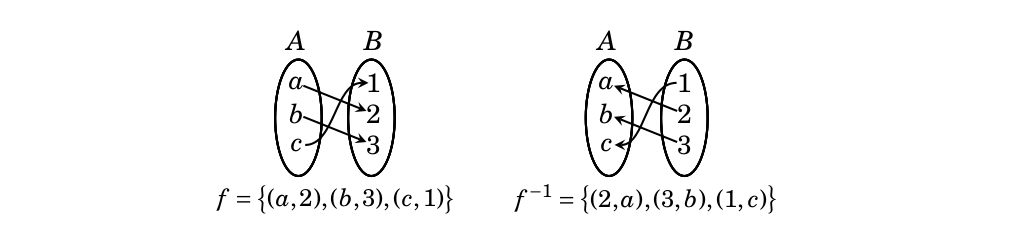
\includegraphics{../../png/InverseExample1.png}

\vfill

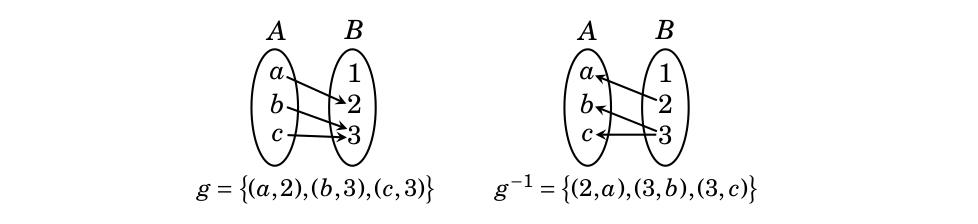
\includegraphics{../../png/InverseExample2.png}

\vfill\eject

\hypertarget{the-inverse-function-theorem}{%
\subsection{The Inverse Function
Theorem}\label{the-inverse-function-theorem}}

\textbf{Theorem:} Let \(F\subset A\times B\) be a function. The inverse
relation \(F^{-1}\subset B\times A\) is also a function if and only if
\(F\) is bijective.

\vfill\eject

\hypertarget{inverse-functions-definition}{%
\subsection{Inverse functions
(definition)}\label{inverse-functions-definition}}

\textbf{Definition:} If \(f:A\to B\) is bijective, then its
\textbf{inverse} is the function \[f^{-1}:B\to A.\] We have \[
f^{-1}\circ f:A\to A = i_A.
\] and \[
f\circ f^{-1}:B\to B = i_B
\]

\end{document}
